\documentclass{beamer}
\usepackage{array}
\usepackage{mathtools}
\usepackage[normalem]{ulem}
\usepackage{tikz}
\usetikzlibrary{arrows}
\usetikzlibrary{overlay-beamer-styles}
\usetikzlibrary{positioning}
\usetikzlibrary{shapes, shapes.geometric, positioning}
\usetikzlibrary{calc,intersections}
\usepackage{tkz-euclide}
\usetikzlibrary{through}


\usepackage{pgfmath}
\usepackage{pgfplots}



\usepackage{amsmath}
\usepackage{amsfonts}
\usepackage{verbatim}
\usepackage{arcs}
\usepackage{setspace}
\usepackage{hyperref}

%\usepackage{enumerate}
%\usepackage{enumitem}
%\setlist{noitemsep}

\usepackage{listings}
\lstset{language=python}

\usepackage{array, multirow, bigdelim}
\usepackage{makeidx}

\setbeamertemplate{navigation symbols}{}
\usetheme{CambridgeUS}
\usecolortheme{Vermillion}

\usepackage{adjustbox}


%\DeclareMathOperator*{\argmax}{argmax}
\DeclareMathOperator*{\argmax}{arg\,max}
\DeclareMathOperator*{\argmin}{arg\,min}

\definecolor{codegreen}{rgb}{0,0.6,0}
\definecolor{codegray}{rgb}{0.5,0.5,0.5}
\definecolor{codepurple}{rgb}{0.58,0,0.82}
\definecolor{backcolour}{rgb}{0.95,0.95,0.92}

\lstdefinestyle{mystyle}{
    backgroundcolor=\color{white},   
    commentstyle=\color{codegreen},
    keywordstyle=\color{magenta},
    numberstyle=\tiny\color{codegray},
    stringstyle=\color{codepurple},
    basicstyle=\ttfamily,
    breakatwhitespace=false,         
    breaklines=true,                 
    captionpos=t,                    
    keepspaces=true,                 
    numbers=left,                    
    numbersep=5pt,                  
    showspaces=false,                
    showstringspaces=false,
    showtabs=false,                  
    tabsize=2
}

\AtBeginSection[] {
    \begin{frame}<beamer>{Outline}
    \tableofcontents[currentsection]
    \end{frame}
}

%%%%%
\title{\LaTeX: What? Why? and How?}
\subtitle{CSCE 595 Presentation}
\author{Brad Burkman}
\institute[LSMSA]{Louisiana School for Math, Science, and the Arts}
\date{31 January 2020}

\begin{document}
\logo{\includegraphics[height=1.0cm]{AcademicHorizontal_0.jpg}\hspace{12pt}}
\newcommand{\nologo}{\setbeamertemplate{logo}{}} 


\begin{frame}[t]
	\Large
	\maketitle
\end{frame}

% TOC
\begin{frame}[t]
	\Large
	\tableofcontents[hideallsubsections]
\end{frame}



% Overview
\section{Overview}

\subsection{Procedural Markup Language}
\begin{frame}[t, fragile]
	\frametitle{Procedural Markup Language}
\Large


\verb|$$\frac{-b \pm \sqrt{b^2 - 4ac}}{2a}$$|

$$\frac{-b \pm \sqrt{b^2 - 4ac}}{2a}$$

\begin{itemize}
	\item NOT WYSIWIG, ``What You See Is What You Get''
	\item Steep Learning Curve
	\item Open Source, Free
	
	``Free as in Free Speech and Free Beer''
	\item Lots of user-created libraries and packages
	\item Programming Language Stuff
\end{itemize} 
\end{frame}

\subsection{History}
\begin{frame}[t]
	\frametitle{History}
\Large

\begin{itemize}
	\item Donald Knuth, \TeX, 1978
	\item Leslie Lamport, \LaTeX, 1983
	\item Last Stable Release, \LaTeX2$\epsilon$, 1994
	\item MathType (WYSIWIG GUI for Word), 1987
\end{itemize}

\end{frame}

\subsection{Examples in GitHub Repo}
\begin{frame}[t]
	\frametitle{Examples in GitHub Repo}
\Large

\begin{itemize}
	\item This Presentation
	\item Paper in ACL Format
	\item Poster
	\item Book
\end{itemize}

\end{frame}




\section{Examples}
\subsection{Math}
% Equations
\begin{frame}[t, fragile]
	\frametitle{Equations}
\Large

\verb|$$\int_a^b f(x) dx = \lim_{n \to \infty}|

\qquad \verb| \sum_{i=1}^n f(x^*_i) \Delta x$$|

$$\int_a^b f(x) dx = \lim_{n \to \infty} \sum_{i=1}^n f(x^*_i) \Delta x$$

\verb|$\int_a^b f(x) dx = \lim_{n \to \infty}|

\qquad \verb| \sum_{i=1}^n f(x^*_i) \Delta x$|

\begin{center}
$\int_a^b f(x) dx = \lim_{n \to \infty} \sum_{i=1}^n f(x^*_i) \Delta x$
\end{center}
\end{frame}

% Aligned Equations
\begin{frame}[t, fragile]
	\frametitle{Aligned Equations}
\Large

\begin{columns}[T]
\begin{column}{2in}
\begin{verbatim}



\begin{align*}
    e^{3x+4} &= 2 \cr
    3x+4 &= \ln 2 \cr
    3x &= \ln 2 - 4 \cr
    x &= \frac{\ln 2 - 4}{3} \cr
\end{align*}
\end{verbatim}
\end{column}
\begin{column}{2in}
\begin{align*}
	e^{3x+4} &= 2 \cr
	3x+4 &= \ln 2 \cr
	3x &= \ln 2 - 4 \cr
	x &= \frac{\ln 2 - 4}{3} \cr
\end{align*}
\end{column}
\end{columns}
\end{frame}

% Tables
\subsection{Tables}
\begin{frame}[t, fragile]
	\frametitle{Tabular Environment}
\large
\begin{tabular}{ll|lclc}
\multicolumn{2}{c}{Teacher} & Course & Period & Course & Period \cr\hline
Emily  &  Allen  &  EN300.1  &  13  &  EN300.3  &  14 \cr
Scott  &  Atkins  &  PH240L.1  &  12  &  PH120.2  &  13 \cr
Robert  &  Dalling  &  PH320.1  &  13  &  PH350.1  &  14 \cr
Leo  &  Eisenlohr  &  FL170.1  &  13  &  FL270.1  &  14 \cr
Victor  &  Feske  &  EH122.1  &  13  &  EH122.2  &  14 \cr
\end{tabular}

\begin{verbatim}
\begin{tabular}{ll|lclc}
\multicolumn{2}{c}{Teacher} 
    & Course & Period & Course & Period \cr\hline
Emily & Allen & EN300.1 & 13 &  EN300.3 & 14 \cr
...
\end{tabular}
\end{verbatim}
\end{frame}

% Alignment
\begin{frame}[t, fragile]
	\frametitle{Tables with Math}
\Large

\begin{center}
\begin{tabular}{*5{@{\hspace{4pt}}>{$}r<{$}}}
	2x &+& 15y &=& 6 \cr
	3x &-& 4y &<& 12 \cr 
\end{tabular}
\end{center}

\begin{verbatim}
\begin{tabular}{*5{@{\hspace{4pt}}>{$}r<{$}}}
    2x &+& 15y &=& 6 \cr
    3x &-& 4y &<& 12 \cr 
\end{tabular}
\end{verbatim}
\end{frame}

% Code
\subsection{Code}
\begin{frame}[t]
	\frametitle{Code}
\Large

\lstinputlisting[language=python, caption = Default Style, 
	]{stuff.py}

\end{frame}

\begin{frame}[t]
	\frametitle{Code}
\Large

\lstset{style=mystyle}
\lstinputlisting[language=python, caption = Formatted No Color, 
	backgroundcolor=\color{white},   
	commentstyle=\color{black},
	keywordstyle=\color{black},
	numberstyle=\tiny\color{black},
	stringstyle=\color{black},
	basicstyle=\ttfamily,	
	]{stuff.py}

\end{frame}

\begin{frame}[t]
	\frametitle{Code}
\Large

\lstset{style=mystyle}
\lstinputlisting[caption = Typical Colors]{stuff.py}

\end{frame}

\begin{frame}[t]
	\frametitle{Code}
\Large

\lstset{style=mystyle}
\lstinputlisting[language=python, caption = UL Colors, 
	backgroundcolor=\color{white},   
	commentstyle=\color{black},
	keywordstyle=\color{vermillion},
	numberstyle=\tiny\color{black},
	stringstyle=\color{black},
	basicstyle=\ttfamily,	
	]{stuff.py}

\end{frame}

% Graphs
\subsection{Graphs}

\begin{frame}[t]
	\frametitle{Ti\textit{k}Z}
\Large

Graphics Package for \LaTeX

Ti\textit{k}Z {\it ist kein Zeichenprogramm}

``Ti\textit{k}Z is not a graphing program.''



\end{frame}



\begin{frame}[t, fragile]
	\frametitle{Graphs:  Fall 2018 \#L3}
\Large
\hfil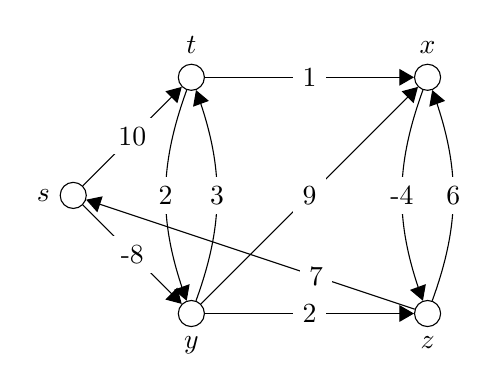
\begin{tikzpicture}[x=15mm, y=15mm]
	\node [circle, draw, label=left:$s$] (s) at (0,0) {};
	\node [circle, draw, label=above:$t$] (t) at (1,1) {};
	\node [circle, draw, label=above:$x$] (x) at (3,1) {};
	\node [circle, draw, label=below:$y$] (y) at (1,-1) {};
	\node [circle, draw, label=below:$z$] (z) at (3,-1) {};
	\foreach \from/\to/\weight in {s/t/10, s/y/-8, t/x/1, y/x/9, y/z/2}
		\draw [-triangle 60] (\from) -- (\to) node [midway, rectangle, fill=white] {\weight};
	\foreach \from/\to/\weight in {z/s/7}
		\draw [-triangle 60] (\from) -- (\to) node [pos=0.3, rectangle, fill=white] {\weight};
	\foreach \from/\to/\weight in {t/y/2, y/t/3, x/z/-4, z/x/6}
		\draw [bend right=20, -triangle 60] (\from) to node [midway, rectangle, fill=white] {\weight} (\to);
\end{tikzpicture}

\lstset{style=mystyle}
\lstinputlisting[language=TeX, tabsize=2, linerange={1-2}]{Graph_Code.tex}
\end{frame}

\begin{frame}[t, fragile]
	\frametitle{}
\Large
\hfil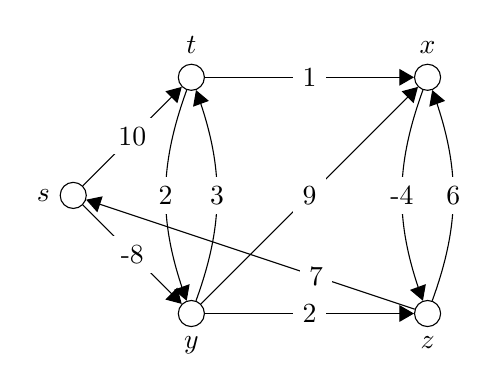
\begin{tikzpicture}[x=15mm, y=15mm]
	\node [circle, draw, label=left:$s$] (s) at (0,0) {};
	\node [circle, draw, label=above:$t$] (t) at (1,1) {};
	\node [circle, draw, label=above:$x$] (x) at (3,1) {};
	\node [circle, draw, label=below:$y$] (y) at (1,-1) {};
	\node [circle, draw, label=below:$z$] (z) at (3,-1) {};
	\foreach \from/\to/\weight in {s/t/10, s/y/-8, t/x/1, y/x/9, y/z/2}
		\draw [-triangle 60] (\from) -- (\to) node [midway, rectangle, fill=white] {\weight};
	\foreach \from/\to/\weight in {z/s/7}
		\draw [-triangle 60] (\from) -- (\to) node [pos=0.3, rectangle, fill=white] {\weight};
	\foreach \from/\to/\weight in {t/y/2, y/t/3, x/z/-4, z/x/6}
		\draw [bend right=20, -triangle 60] (\from) to node [midway, rectangle, fill=white] {\weight} (\to);
\end{tikzpicture}

\lstset{style=mystyle}
\lstinputlisting[language=TeX, tabsize=2, linerange={7-8}]{Graph_Code.tex}
\end{frame}

\begin{frame}[t, fragile]
	\frametitle{}
\Large
\hfil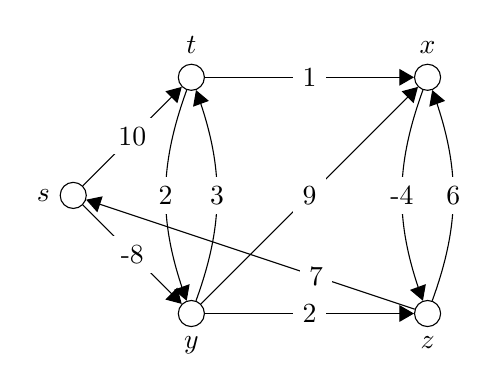
\begin{tikzpicture}[x=15mm, y=15mm]
	\node [circle, draw, label=left:$s$] (s) at (0,0) {};
	\node [circle, draw, label=above:$t$] (t) at (1,1) {};
	\node [circle, draw, label=above:$x$] (x) at (3,1) {};
	\node [circle, draw, label=below:$y$] (y) at (1,-1) {};
	\node [circle, draw, label=below:$z$] (z) at (3,-1) {};
	\foreach \from/\to/\weight in {s/t/10, s/y/-8, t/x/1, y/x/9, y/z/2}
		\draw [-triangle 60] (\from) -- (\to) node [midway, rectangle, fill=white] {\weight};
	\foreach \from/\to/\weight in {z/s/7}
		\draw [-triangle 60] (\from) -- (\to) node [pos=0.3, rectangle, fill=white] {\weight};
	\foreach \from/\to/\weight in {t/y/2, y/t/3, x/z/-4, z/x/6}
		\draw [bend right=20, -triangle 60] (\from) to node [midway, rectangle, fill=white] {\weight} (\to);
\end{tikzpicture}

\lstset{style=mystyle}
\lstinputlisting[language=TeX, tabsize=2, linerange={11-12}]{Graph_Code.tex}
\end{frame}


\subsection{Graphing}

\begin{frame}[t]
	\frametitle{Harmonic Series}
\Large

\only<1-2>{
\hfil$\displaystyle1 + \frac{1}{2} + \frac{1}{3} + \frac{1}{4} + \frac{1}{5} + \cdots = \lim_{n \to \infty}\sum_{r=1}^n \frac{1}{r}$

}
\only<3->{
\hfil$\displaystyle1 + \frac{1}{2} + \frac{1}{3} + \frac{1}{4} + \frac{1}{5} + \cdots + \frac{1}{n} = \sum_{r=1}^n \frac{1}{r}$

}

\only<1-3>{\vskip 12pt This series does not converge.}

\only<2-3>{
	\vskip 12pt
	Source of my confusion:  In our work, $n$ is finite.
}

\only<4->{
\begin{tikzpicture}[x=8mm,y=8mm]
	\draw [triangle 60-triangle 60] (-1,0) -- (11,0);
	\draw [triangle 60-triangle 60] (0,-1) -- (0,4.5);
	\foreach \i in {1,2,...,10}{
		\draw (\i,.2) -- (\i,-.2) node [below] {\i};
	}
	\foreach \i in {1,2,3}{
		\draw (0.2,\i) -- (-0.2,\i) node [left] {\i};
	}
	\fill (1,1.000000) circle (2pt);
\fill (2,1.500000) circle (2pt);
\fill (3,1.833333) circle (2pt);
\fill (4,2.083333) circle (2pt);
\fill (5,2.283333) circle (2pt);
\fill (6,2.450000) circle (2pt);
\fill (7,2.592857) circle (2pt);
\fill (8,2.717857) circle (2pt);
\fill (9,2.828968) circle (2pt);
\fill (10,2.928968) circle (2pt);
\draw (1,1.000000) -- (2,1.500000) -- (3,1.833333) -- (4,2.083333) -- (5,2.283333) -- (6,2.450000) -- (7,2.592857) -- (8,2.717857) -- (9,2.828968) -- (10,2.928968);

	\path (10,3.0) node [right] {Partial Sum};
	\only<5->{
	\fill [vermillion](1,0.000000) circle (2pt);
\fill [vermillion](2,0.693147) circle (2pt);
\fill [vermillion](3,1.098612) circle (2pt);
\fill [vermillion](4,1.386294) circle (2pt);
\fill [vermillion](5,1.609438) circle (2pt);
\fill [vermillion](6,1.791759) circle (2pt);
\fill [vermillion](7,1.945910) circle (2pt);
\fill [vermillion](8,2.079442) circle (2pt);
\fill [vermillion](9,2.197225) circle (2pt);
\fill [vermillion](10,2.302585) circle (2pt);
\draw [vermillion] (1,0.000000) -- (2,0.693147) -- (3,1.098612) -- (4,1.386294) -- (5,1.609438) -- (6,1.791759) -- (7,1.945910) -- (8,2.079442) -- (9,2.197225) -- (10,2.302585);

	\path (10,2.0) node [vermillion,right] {$y = \log(n)$};
	}
	\only<7>{
		\draw [vermillion](1,1.000000) circle (2pt);
\draw [vermillion](2,1.693147) circle (2pt);
\draw [vermillion](3,2.098612) circle (2pt);
\draw [vermillion](4,2.386294) circle (2pt);
\draw [vermillion](5,2.609438) circle (2pt);
\draw [vermillion](6,2.791759) circle (2pt);
\draw [vermillion](7,2.945910) circle (2pt);
\draw [vermillion](8,3.079442) circle (2pt);
\draw [vermillion](9,3.197225) circle (2pt);
\draw [vermillion](10,3.302585) circle (2pt);
\draw [vermillion] (1,1.000000) -- (2,1.693147) -- (3,2.098612) -- (4,2.386294) -- (5,2.609438) -- (6,2.791759) -- (7,2.945910) -- (8,3.079442) -- (9,3.197225) -- (10,3.302585);

	\path (2,3.5) node [vermillion,right] {$y = \log(n)+1$};
	}
	
\end{tikzpicture}
}

%\vskip 6pt
 
\only<6>{
	$\displaystyle\frac{dy}{dx} = y, \ (0,1) \qquad \frac{dy}{dx} = \frac{1}{x}, \ (1,0)$
}
\only<7>{
%	$\displaystyle\frac{dy}{dx} = y, \ (0,1) \qquad \frac{dy}{dx} = \frac{1}{x}, \ (1,0)$
	$\displaystyle\frac{dy}{dx} = y, \ (0,1) \qquad \frac{dy}{dx} = \frac{1}{x}, \ (1,0) \ {\color{vermillion}(1,1)}$
}

\end{frame}

\begin{frame}[t]
	\frametitle{}
\Large

\begin{tikzpicture}[domain=0.8:5.5,x=20mm,y=20mm]
	\only<3>{
		\foreach \i in {1,2,3,4}{
			\fill [vermillion] (\i,0) rectangle ({\i+1},{1/\i});
		}
	}
	\only<2->{
	\fill [black, domain=1:4, variable=\x]
  		(1, 0)  -- plot ({\x}, {1/\x})  -- (4, 0)  -- cycle;
	}
	\only<3>{
		\foreach \i in {1,2,3,4}{
			\draw [vermillion] (\i,0) rectangle ({\i+1},{1/\i});
		}
	}
	\only<4>{
	\foreach \i in {1,2,3,4}{
		\fill [vermillion] ({\i-1},0) rectangle ({\i},{1/\i});
	}
	\fill [vermillion] (1,0) rectangle (2,{1/5});
	}

	\draw [triangle 60-triangle 60] (-0.5,0) -- (5.5,0);
	\draw [triangle 60-triangle 60] (0,-0.3) -- (0,1.5);
	\foreach \i in {1,2,...,5}{
		\draw (\i,.1) -- (\i,-.1) node [below] {\i};
	}
	\foreach \i in {1}{
		\draw (0.2,\i) -- (-0.2,\i) node [left] {\i};
	}
	\draw[color=black, ultra thick, triangle 60-triangle 60] plot[id=sin] function{1/x};
	\path (0.8,1.25) node[above] {$y=1/x$};
	\only<2>{\path (3.5,1) node {$\log(4)$};}
	\only<3>{\path (3.5,1) node {$\displaystyle\log(4)< \frac{1}{1} + \frac{1}{2} + \frac{1}{3} + \frac{1}{4}$};}
	\only<4>{\path (3.5,1) node {$\displaystyle\left(\frac{1}{1} + \frac{1}{2} + \frac{1}{3} + \frac{1}{4}\right) - 1 < \log(4)$};}
	
	\end{tikzpicture}
	\vskip -12pt
	
	\only<3>{
		$$\log(n)<\sum_{r=1}^n \frac{1}{r}$$
	}
	\only<4>{
		$$  \sum_{r=1}^n \frac{1}{r} - 1 \ < \ \log(n)$$
	}
	\only<5>{
		$$\log(n)  \ < \ \sum_{r=1}^n \frac{1}{r} \ < \ \log(n)+1$$
	}
	
\end{frame}

\begin{frame}[t]
	\frametitle{}
\Large

\begin{tikzpicture}[x=0.004mm,y=5.5mm]
	\draw [triangle 60-triangle 60] (-2000,0) -- (22000,0);
	\draw [triangle 60-triangle 60] (0,-1) -- (0,11);
	\foreach \i in {1,2,3,...,10}{
		\draw (400,\i) -- (-400,\i) node [left] {\i};
	}
	\draw (5000,.2) -- (5000,-.2) node [below] {5000};
	\draw (10000,.2) -- (10000,-.2) node [below] {10000};
	\draw (15000,.2) -- (15000,-.2) node [below] {15000};
	\draw (20000,.2) -- (20000,-.2) node [below] {20000};
	\fill (2,1.500000) circle (2pt);
\fill (402,6.574911) circle (2pt);
\fill (802,7.264948) circle (2pt);
\fill (1202,7.669374) circle (2pt);
\fill (1602,7.956536) circle (2pt);
\fill (2002,8.179367) circle (2pt);
\fill (2402,8.361481) circle (2pt);
\fill (2802,8.515483) circle (2pt);
\fill (3202,8.648903) circle (2pt);
\fill (3602,8.766599) circle (2pt);
\fill (4002,8.871890) circle (2pt);
\fill (4402,8.967144) circle (2pt);
\fill (4802,9.054108) circle (2pt);
\fill (5202,9.134110) circle (2pt);
\fill (5602,9.208184) circle (2pt);
\fill (6002,9.277147) circle (2pt);
\fill (6402,9.341659) circle (2pt);
\fill (6802,9.402261) circle (2pt);
\fill (7202,9.459399) circle (2pt);
\fill (7602,9.513448) circle (2pt);
\fill (8002,9.564725) circle (2pt);
\fill (8402,9.613500) circle (2pt);
\fill (8802,9.660007) circle (2pt);
\fill (9202,9.704446) circle (2pt);
\fill (9602,9.746994) circle (2pt);
\fill (10002,9.787806) circle (2pt);
\fill (10402,9.827017) circle (2pt);
\fill (10802,9.864749) circle (2pt);
\fill (11202,9.901108) circle (2pt);
\fill (11602,9.936192) circle (2pt);
\fill (12002,9.970086) circle (2pt);
\fill (12402,10.002869) circle (2pt);
\fill (12802,10.034611) circle (2pt);
\fill (13202,10.065377) circle (2pt);
\fill (13602,10.095225) circle (2pt);
\fill (14002,10.124207) circle (2pt);
\fill (14402,10.152373) circle (2pt);
\fill (14802,10.179767) circle (2pt);
\fill (15202,10.206431) circle (2pt);
\fill (15602,10.232402) circle (2pt);
\fill (16002,10.257716) circle (2pt);
\fill (16402,10.282405) circle (2pt);
\fill (16802,10.306499) circle (2pt);
\fill (17202,10.330026) circle (2pt);
\fill (17602,10.353012) circle (2pt);
\fill (18002,10.375482) circle (2pt);
\fill (18402,10.397457) circle (2pt);
\fill (18802,10.418961) circle (2pt);
\fill (19202,10.440011) circle (2pt);
\fill (19602,10.460628) circle (2pt);
\draw (2,1.500000) -- (402,6.574911) -- (802,7.264948) -- (1202,7.669374) -- (1602,7.956536) -- (2002,8.179367) -- (2402,8.361481) -- (2802,8.515483) -- (3202,8.648903) -- (3602,8.766599) -- (4002,8.871890) -- (4402,8.967144) -- (4802,9.054108) -- (5202,9.134110) -- (5602,9.208184) -- (6002,9.277147) -- (6402,9.341659) -- (6802,9.402261) -- (7202,9.459399) -- (7602,9.513448) -- (8002,9.564725) -- (8402,9.613500) -- (8802,9.660007) -- (9202,9.704446) -- (9602,9.746994) -- (10002,9.787806) -- (10402,9.827017) -- (10802,9.864749) -- (11202,9.901108) -- (11602,9.936192) -- (12002,9.970086) -- (12402,10.002869) -- (12802,10.034611) -- (13202,10.065377) -- (13602,10.095225) -- (14002,10.124207) -- (14402,10.152373) -- (14802,10.179767) -- (15202,10.206431) -- (15602,10.232402) -- (16002,10.257716) -- (16402,10.282405) -- (16802,10.306499) -- (17202,10.330026) -- (17602,10.353012) -- (18002,10.375482) -- (18402,10.397457) -- (18802,10.418961) -- (19202,10.440011) -- (19602,10.460628);

	\path (20000,10.5) node [right] {Partial Sum};
	\fill [vermillion](1,0.000000) circle (2pt);
\fill [vermillion](401,5.993961) circle (2pt);
\fill [vermillion](801,6.685861) circle (2pt);
\fill [vermillion](1201,7.090910) circle (2pt);
\fill [vermillion](1601,7.378384) circle (2pt);
\fill [vermillion](2001,7.601402) circle (2pt);
\fill [vermillion](2401,7.783641) circle (2pt);
\fill [vermillion](2801,7.937732) circle (2pt);
\fill [vermillion](3201,8.071219) circle (2pt);
\fill [vermillion](3601,8.188967) circle (2pt);
\fill [vermillion](4001,8.294300) circle (2pt);
\fill [vermillion](4401,8.389587) circle (2pt);
\fill [vermillion](4801,8.476580) circle (2pt);
\fill [vermillion](5201,8.556606) circle (2pt);
\fill [vermillion](5601,8.630700) circle (2pt);
\fill [vermillion](6001,8.699681) circle (2pt);
\fill [vermillion](6401,8.764210) circle (2pt);
\fill [vermillion](6801,8.824825) circle (2pt);
\fill [vermillion](7201,8.881975) circle (2pt);
\fill [vermillion](7601,8.936035) circle (2pt);
\fill [vermillion](8001,8.987322) circle (2pt);
\fill [vermillion](8401,9.036106) circle (2pt);
\fill [vermillion](8801,9.082621) circle (2pt);
\fill [vermillion](9201,9.127067) circle (2pt);
\fill [vermillion](9601,9.169623) circle (2pt);
\fill [vermillion](10001,9.210440) circle (2pt);
\fill [vermillion](10401,9.249657) circle (2pt);
\fill [vermillion](10801,9.287394) circle (2pt);
\fill [vermillion](11201,9.323758) circle (2pt);
\fill [vermillion](11601,9.358847) circle (2pt);
\fill [vermillion](12001,9.392745) circle (2pt);
\fill [vermillion](12401,9.425532) circle (2pt);
\fill [vermillion](12801,9.457279) circle (2pt);
\fill [vermillion](13201,9.488048) circle (2pt);
\fill [vermillion](13601,9.517899) circle (2pt);
\fill [vermillion](14001,9.546884) circle (2pt);
\fill [vermillion](14401,9.575053) circle (2pt);
\fill [vermillion](14801,9.602450) circle (2pt);
\fill [vermillion](15201,9.629116) circle (2pt);
\fill [vermillion](15601,9.655090) circle (2pt);
\fill [vermillion](16001,9.680406) circle (2pt);
\fill [vermillion](16401,9.705098) circle (2pt);
\fill [vermillion](16801,9.729194) circle (2pt);
\fill [vermillion](17201,9.752723) circle (2pt);
\fill [vermillion](17601,9.775711) circle (2pt);
\fill [vermillion](18001,9.798183) circle (2pt);
\fill [vermillion](18401,9.820160) circle (2pt);
\fill [vermillion](18801,9.841665) circle (2pt);
\fill [vermillion](19201,9.862718) circle (2pt);
\fill [vermillion](19601,9.883336) circle (2pt);
\draw [vermillion] (1,0.000000) -- (401,5.993961) -- (801,6.685861) -- (1201,7.090910) -- (1601,7.378384) -- (2001,7.601402) -- (2401,7.783641) -- (2801,7.937732) -- (3201,8.071219) -- (3601,8.188967) -- (4001,8.294300) -- (4401,8.389587) -- (4801,8.476580) -- (5201,8.556606) -- (5601,8.630700) -- (6001,8.699681) -- (6401,8.764210) -- (6801,8.824825) -- (7201,8.881975) -- (7601,8.936035) -- (8001,8.987322) -- (8401,9.036106) -- (8801,9.082621) -- (9201,9.127067) -- (9601,9.169623) -- (10001,9.210440) -- (10401,9.249657) -- (10801,9.287394) -- (11201,9.323758) -- (11601,9.358847) -- (12001,9.392745) -- (12401,9.425532) -- (12801,9.457279) -- (13201,9.488048) -- (13601,9.517899) -- (14001,9.546884) -- (14401,9.575053) -- (14801,9.602450) -- (15201,9.629116) -- (15601,9.655090) -- (16001,9.680406) -- (16401,9.705098) -- (16801,9.729194) -- (17201,9.752723) -- (17601,9.775711) -- (18001,9.798183) -- (18401,9.820160) -- (18801,9.841665) -- (19201,9.862718) -- (19601,9.883336);

	\path (20000,9.5)node [vermillion,right] {$y = \log(n)$};
	\path (20000,11.5)node [vermillion,right] {$y = \log(n)+1$};
	\draw [vermillion](1,1.000000) circle (2pt);
\draw [vermillion](401,6.993961) circle (2pt);
\draw [vermillion](801,7.685861) circle (2pt);
\draw [vermillion](1201,8.090910) circle (2pt);
\draw [vermillion](1601,8.378384) circle (2pt);
\draw [vermillion](2001,8.601402) circle (2pt);
\draw [vermillion](2401,8.783641) circle (2pt);
\draw [vermillion](2801,8.937732) circle (2pt);
\draw [vermillion](3201,9.071219) circle (2pt);
\draw [vermillion](3601,9.188967) circle (2pt);
\draw [vermillion](4001,9.294300) circle (2pt);
\draw [vermillion](4401,9.389587) circle (2pt);
\draw [vermillion](4801,9.476580) circle (2pt);
\draw [vermillion](5201,9.556606) circle (2pt);
\draw [vermillion](5601,9.630700) circle (2pt);
\draw [vermillion](6001,9.699681) circle (2pt);
\draw [vermillion](6401,9.764210) circle (2pt);
\draw [vermillion](6801,9.824825) circle (2pt);
\draw [vermillion](7201,9.881975) circle (2pt);
\draw [vermillion](7601,9.936035) circle (2pt);
\draw [vermillion](8001,9.987322) circle (2pt);
\draw [vermillion](8401,10.036106) circle (2pt);
\draw [vermillion](8801,10.082621) circle (2pt);
\draw [vermillion](9201,10.127067) circle (2pt);
\draw [vermillion](9601,10.169623) circle (2pt);
\draw [vermillion](10001,10.210440) circle (2pt);
\draw [vermillion](10401,10.249657) circle (2pt);
\draw [vermillion](10801,10.287394) circle (2pt);
\draw [vermillion](11201,10.323758) circle (2pt);
\draw [vermillion](11601,10.358847) circle (2pt);
\draw [vermillion](12001,10.392745) circle (2pt);
\draw [vermillion](12401,10.425532) circle (2pt);
\draw [vermillion](12801,10.457279) circle (2pt);
\draw [vermillion](13201,10.488048) circle (2pt);
\draw [vermillion](13601,10.517899) circle (2pt);
\draw [vermillion](14001,10.546884) circle (2pt);
\draw [vermillion](14401,10.575053) circle (2pt);
\draw [vermillion](14801,10.602450) circle (2pt);
\draw [vermillion](15201,10.629116) circle (2pt);
\draw [vermillion](15601,10.655090) circle (2pt);
\draw [vermillion](16001,10.680406) circle (2pt);
\draw [vermillion](16401,10.705098) circle (2pt);
\draw [vermillion](16801,10.729194) circle (2pt);
\draw [vermillion](17201,10.752723) circle (2pt);
\draw [vermillion](17601,10.775711) circle (2pt);
\draw [vermillion](18001,10.798183) circle (2pt);
\draw [vermillion](18401,10.820160) circle (2pt);
\draw [vermillion](18801,10.841665) circle (2pt);
\draw [vermillion](19201,10.862718) circle (2pt);
\draw [vermillion](19601,10.883336) circle (2pt);
\draw [vermillion] (1,1.000000) -- (401,6.993961) -- (801,7.685861) -- (1201,8.090910) -- (1601,8.378384) -- (2001,8.601402) -- (2401,8.783641) -- (2801,8.937732) -- (3201,9.071219) -- (3601,9.188967) -- (4001,9.294300) -- (4401,9.389587) -- (4801,9.476580) -- (5201,9.556606) -- (5601,9.630700) -- (6001,9.699681) -- (6401,9.764210) -- (6801,9.824825) -- (7201,9.881975) -- (7601,9.936035) -- (8001,9.987322) -- (8401,10.036106) -- (8801,10.082621) -- (9201,10.127067) -- (9601,10.169623) -- (10001,10.210440) -- (10401,10.249657) -- (10801,10.287394) -- (11201,10.323758) -- (11601,10.358847) -- (12001,10.392745) -- (12401,10.425532) -- (12801,10.457279) -- (13201,10.488048) -- (13601,10.517899) -- (14001,10.546884) -- (14401,10.575053) -- (14801,10.602450) -- (15201,10.629116) -- (15601,10.655090) -- (16001,10.680406) -- (16401,10.705098) -- (16801,10.729194) -- (17201,10.752723) -- (17601,10.775711) -- (18001,10.798183) -- (18401,10.820160) -- (18801,10.841665) -- (19201,10.862718) -- (19601,10.883336);

	\fill [black] (12000,10) circle (6pt) node [above left] {$(12000,10)$};
	\path (15000,8) node [below] {
		\begin{minipage}{4in}
\only<2>{
\vskip 24pt
Let $N$ be the total number of words in the corpus.

Let $n$ be the number of unique words.
}
\only<2-3>{
$$N = \sum_{r=1}^n f_r$$
}
\only<3-4>{
$$N = \sum_{r=1}^n f_r = \sum_{r=1}^n \frac{NA}{r} =  NA \sum_{r=1}^n \frac{1}{r}  \approx NA\log(n)$$
}
\only<4-5>{
$$N = NA \sum_{r=1}^n \frac{1}{r}  \approx NA\log(n)$$
}
\only<5-6>{
$$1 = A \sum_{r=1}^n \frac{1}{r}  \approx A\log(n)$$
}
\only<6-8>{
$$A = \frac{1}{\sum_{r=1}^n \frac{1}{r}}  \approx \frac{1}{log(n)}$$
}
\only<7-8>{

	If $n \approx 12000$, then $\displaystyle A \approx 1/10$.
}
\only<8>{

\vskip 6pt

	If $n \approx 4500$, then $A \approx 1/9$.

	If $n \approx 33000$, then $A \approx 1/11$.
	
}


		\end{minipage}
	};
\end{tikzpicture}
\end{frame}



\section{Powerful Techniques}
% Generating LaTeX
\subsection{Code Output can be \LaTeX \ Input}

\begin{frame}[t]
	\frametitle{Code Output can be \LaTeX \ Input}
\Large
\lstset{style=mystyle}
\lstinputlisting[
	backgroundcolor=\color{white},   
	commentstyle=\color{black},
	keywordstyle=\color{vermillion},
	numberstyle=\tiny\color{black},
	stringstyle=\color{black},
	basicstyle=\ttfamily,	
]{Graph03.py}
\end{frame}

\begin{frame}[t]
	\frametitle{}
\Large
\lstset{style=mystyle}
\lstinputlisting[language=TeX,     tabsize=2]{Graph03.tex}
\end{frame}

\begin{frame}[t]
	\frametitle{}
\Large
\lstset{style=mystyle}
\lstinputlisting[language=TeX,     tabsize=2, linerange={117-117,127-128,133-133}]{Burkman_561_NLTK.tex}

\end{frame}

\begin{frame}[t]
	\frametitle{\LaTeX \ Input is Plain Text}
\Large
\begin{itemize}
	\item Code Output can be \LaTeX \ Input
	\item Structured Documents
	\begin{itemize}
		\item Multi-File
		\item Chapters, Sections, Subsections
		\item Table of Contents
		\item Index
		\item Bibliography
	\end{itemize}
	\item Git
	\begin{itemize}
		\item Version Control
		\item Collaboration
	\end{itemize}
\end{itemize}


\end{frame}



%%%%%%%%%%%%
%
% End
%
%%%%%%%%%%%

\end{document}
%%%%%%%%%
%
% Generic structures
%
%%%%%%%%%%%



\begin{frame}[t]
	\frametitle{}
\Large

\end{frame}


\begin{enumerate}
	\item 
\end{enumerate}


\begin{itemize}
	\item 
\end{itemize}


\begin{tabular}{@{}rl}
	Given: & \cr
	Prove: & \cr
\end{tabular}


\begin{tikzpicture}[x=10mm, y=10mm]
	\coordinate () at ();
	\path () node [] {$$};
\end{tikzpicture}


\begin{tabular}{*5{@{\hspace{5pt}}>{$\displaystyle}r<{$\vrule width 0pt height 12pt depth 4pt}}}

\end{tabular}

